%
% Copyright 2018 Markus Borg, Lund University
%
% This work is licensed under a Creative Commons Attribution-ShareAlike 4.0 International License.
% See http://creativecommons.org/licenses/by-sa/4.0/
%
% The dodument is based on a LaTeX template developed by Jean-Philippe Eisenbarth
% https://github.com/jpeisenbarth/SRS-Tex
%
\documentclass{scrreprt}
\usepackage{graphicx}
\usepackage{listings}
\usepackage{underscore}
\usepackage[bookmarks=true]{hyperref}
\usepackage[utf8]{inputenc}
\usepackage[english]{babel}
\hypersetup{
    bookmarks=false,    % show bookmarks bar?
    pdftitle={Lab 3},    % title
    pdfauthor={Markus Borg},                     % author
    pdfsubject={TeX and LaTeX},                        % subject of the document
    pdfkeywords={TeX, LaTeX, graphics, images}, % list of keywords
    colorlinks=true,       % false: boxed links; true: colored links
    linkcolor=blue,       % color of internal links
    citecolor=black,       % color of links to bibliography
    filecolor=black,        % color of file links
    urlcolor=purple,        % color of external links
    linktoc=page            % only page is linked
}%
\def\myversion{0.2 }
\date{}
%\title
\usepackage{hyperref}
\begin{document}

\begin{flushright}
    \rule{16cm}{5pt}\vskip1cm
    \begin{bfseries}
    	\LARGE{ETSA02-ADM-LAB2}\\
    	\vspace{1.5cm}
        \Huge{Lab 3}\\
        \vspace{0.5cm}
        Automated system testing\\
        \vspace{0.5cm}
        with RobotTestBed\\
        \vspace{1.5cm}
        \LARGE{Version \myversion approved}\\
        \vspace{1.5cm}
        Prepared by Markus Borg\\
        %\vspace{1.5cm}
        Dept. of Computer Science, Lund University\\
        \vspace{1.5cm}
        \today\\
    \end{bfseries}
\end{flushright}

%\tableofcontents

\chapter*{Revision History}

\begin{center}
    \begin{tabular}{|c|c|c|c|}
        \hline
	    Name & Date & Reason For Changes & Version\\
        \hline
	    Markus Borg & 2018-03-21 & Initial draft. & 0.1\\
        \hline
        Markus Borg & 2018-04-01 & First instructions for the RobotTestBed. & 0.2\\
        \hline
        Markus Borg & 2018-04-04 & Drafted introduction section. & 0.3\\
        \hline
    \end{tabular}
\end{center}

\chapter{Introduction}
During Lab 3 you will continue working with automated testing of Basic Melee Bot. You will still use the JUnit framework to drive the test automation, but your test design will leave the unit level to instead target robot behavior on the system level. To enable such testing, you will work with the Robocode plug-in RobotTestBed. Furthermore, you will design test cases to verify quality requirements regarding the battle performance of Basic Melee Bot. More specifically, Lab 3 covers:

\begin{itemize}
\item Working with the RobotTestBed plugin.
\item Designing JUnit test cases for system testing.
\item Designing JUnit test cases for testing quality requirements.
\end{itemize}

\chapter{Before the lab}
The source code required for Lab 3 is available on GitHub:\\https://github.com/lunduniversity/introsofteng\\\\
If you have already cloned the repository, pull the latest source code to make sure you work with the latest version. If you prefer downloading the code, instead click the button presented in Figure~\ref{fig:github} and choose ``Download ZIP''. For Lab 3, you need the files located in introsofteng-master/project/rumble/labs/lab3/src, including its subfolder: `test'. Rewatch the video ``Lab2_download.avi'' on Google Drive (ETSA02 Everyone/Labs) if you need support.

\begin{figure}
\centering
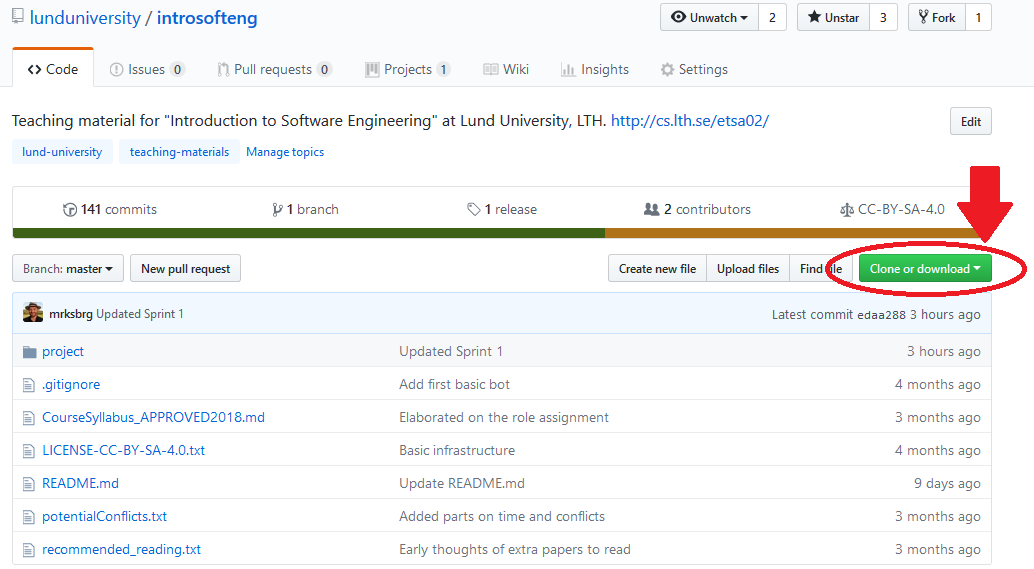
\includegraphics[width=0.99\textwidth]{figures/GitHub.png}
\caption{introsofteng repository on GitHub. The arrow shows the ``Clone or download'' button.}
\label{fig:github}
\end{figure}

Follow these instructions to install the Robocode testing plugin:

\begin{enumerate}
\item Download the latest Robot testing plugin (1.9.3.1) from\\https://sourceforge.net/projects/robocode/files/robocode/1.9.3.1/
\item Add robocode.testing.jar to the Java build path of the project you created in Eclipse. Do this in the same way as when you added robocode.jar.
\item Create a new run configuration for JUnit with RobotTestBed. Do this in the same way as when creating a normal JUnit run configuration, but you must also add -Drobocode.home=$<$PATH TO ROBOCODE$>$ as an argument to the VM.
\end{enumerate}

To get an initial understanding of RobotTestBed, study the simple example TestWallBehavior that follows. The test case verifies that the corresponding robot visits all four corners of the battlefield. RobotTestBed introduces several methods that you can override to add JUnit assertions for testing robot behavior, most importantly:
\begin{itemize}
\item public void onBattleCompleted(BattleCompletedEvent event)
\item public void onRoundStarted(RoundStartedEvent event)
\item public void onRoundEnded(RoundEndedEvent event)
\item public void onTurnEnded(TurnEndedEvent event)
\end{itemize}

During the lab, you will work on designing test cases to verify the four primary features of Basic Melee Bot: 1) Spinning radar, 2) Closest enemy targeting, 3) Non-stop anti-gravity movement, and 4) Wall avoidance. Study the features and the corresponding detailed requirements of Basic Melee Bot in Section~\ref{sec:features}. Also study the quality requirements related to 1-vs-1 battle performance and melee battle performance.

\newpage
\begin{verbatim}
/**
 * Copyright (c) 2001-2018 Mathew A. Nelson and Robocode contributors
 * All rights reserved. This program and the accompanying materials
 * are made available under the terms of the Eclipse Public License v1.0
 * which accompanies this distribution, and is available at
 * http://robocode.sourceforge.net/license/epl-v10.html
 */
package sample;

import static org.junit.Assert.assertTrue;
import robocode.control.events.BattleCompletedEvent;
import robocode.control.events.TurnEndedEvent;
import robocode.control.snapshot.IRobotSnapshot;
import robocode.control.testing.RobotTestBed;

/**
 * Tests that sample.Walls moves to all four corners.
 *
 * @author Philip Johnson (original)
 * @author Pavel Savara (contributor)
 */
public class TestWallBehavior extends RobotTestBed {

	/**
	 * True if the robot visited this corner during the test case.
	 */
	boolean visitedUpperLeft = false;

	/**
	 * True if the robot visited this corner during the test case.
	 */
	boolean visitedUpperRight = false;

	/**
	 * True if the robot visited this corner during the test case.
	 */
	boolean visitedLowerLeft = false;

	/**
	 * True if the robot visited this corner during the test case.
	 */
	boolean visitedLowerRight = false;

	/**
	 * Specifies that SittingDuck and DaCruzer are to be matched up in this test case.
	 *
	 * @return The comma-delimited list of robots in this match.
	 */
	@Override
	public String getRobotNames() {
      return "sample.SittingDuck,sample.Walls";
	}

	/**
	 * This test runs for 1 round.
	 *
	 * @return The number of rounds.
	 */
	@Override
	public int getNumRounds() {
      return 1;
	}

	/**
	 * After each turn, check to see if we're at a corner.
	 * If so, set the corresponding flag.
	 *
	 * @param event Info about the current state of the battle.
	 */
	@Override
	public void onTurnEnded(TurnEndedEvent event) {
      IRobotSnapshot robot = event.getTurnSnapshot().getRobots()[1];
      double xPos = robot.getX();
      double yPos = robot.getY();

      if ((xPos < 40) && (yPos < 40)) {
        visitedUpperLeft = true;
      }
      if ((xPos < 40 && (yPos > (height - 40)))) {
        visitedLowerLeft = true;
      }
      if ((xPos > (width - 40)) && (yPos < 40)) {
        visitedUpperRight = true;
      }
      if ((xPos > (width - 40) && (yPos > (height - 40)))) {
        visitedLowerRight = true;
      }
	}

	/**
	 * After the battle, check to see that we've visited the corners.
	 *
	 * @param event Details about the completed battle.
	 */
	@Override
	public void onBattleCompleted(BattleCompletedEvent
			event) {
      assertTrue("Check UpperLeft", visitedUpperLeft);
      assertTrue("Check LowerLeft", visitedLowerLeft);
      assertTrue("Check UpperRight", visitedUpperRight);
      assertTrue("Check LowerRight", visitedLowerRight);
  }
}
\end{verbatim}

\chapter{Basic Melee Bot Features and Quality Requirements} \label{sec:features}

\section{Feature 1 -- Spinning radar}
BMB shall feature a spinning radar.

\subsection{Description and Priority}
The spinning radar is a simple solution to detect enemy robots by continuously scanning the entire battlefield.\\\\Business priority: \textbf{high}\\
Implementation risk: \textbf{very low}

\subsection{Functional Requirements}
\begin{itemize}
\item[REQ-F1-1] The radar shall scan the battlefield clockwise as long as BMB is operational and the battle is ongoing.
\item[REQ-F1-2] Detected enemy robots shall be stored in an internal data structure. 
\end{itemize}

\section{Feature 2 -- Closest enemy targeting}
BMB shall target and shoot at the closest enemy robot.

\subsection{Description and Priority}
The rationale behind targeting and shooting at the closest enemy is that nearby robots are easier to hit. The solution is simple but useful.\\\\Business priority: \textbf{high}\\
Implementation risk: \textbf{low}

\subsection{Functional Requirements}
\begin{itemize}
\item[REQ-F2-1] BMB shall fire at the closest enemy robot as long as the battle is ongoing.
\item[REQ-F2-2] BMB shall use a constant fire power of 1.
\end{itemize}

\section{Feature 3 -- Non-stop anti-gravity movement}
BMB shall use anti-gravity movement.
	
\subsection{Description and Priority}
Anti-gravity movement is used to keep a distance to certain points on the battlefield. BMB shall use this movement to stay away from enemy robots. Furthermore, BMB shall never stay at one position.\\\\Business priority: \textbf{medium}\\
Implementation risk: \textbf{medium}

\subsection{Functional Requirements}
\begin{itemize}
\item[REQ-F3-1] BMB shall continuously move away from enemy robots.
\item[REQ-F3-2] BMB shall never stay in the same position for more than 10 consecutive turns.
\end{itemize}

\section{Feature 4 -- Wall avoidance}
BMB shall avoid driving into walls.

\subsection{Description and Priority}
Crashing into walls damages robots and forces them into a stop. BMB shall not end up in walls, even when the anti-gravity movement suggests such positions.\\\\Business priority: \textbf{medium}\\
Implementation risk: \textbf{medium}

\subsection{Functional Requirements}
\begin{itemize}
\item[REQ-F4-1] When closer than 40 distance units to a wall, BMB shall alter its course to avoid collision.
\end{itemize}

\section{Quality requirements}
TBD

\subsection{1-vs-1 battle performance}

\subsection{Melee battle performance}

\chapter{At the lab}

%Select your robot class in the Eclipse package explorer. Right-click and select new JUnit test case. Create the new test case. There are several naming conventions, e.g., using the same name as the class under test followed by the suffix `Test' and `Test' as prefix for all methods.
%Software-under-test is the normal name for the object to test, here we use bot-under-test.\\
%Introduce test driven development.

%Inspiration: https://ics613s13.wordpress.com/\\
%Build a robot using maven: https://github.com/bretkikehara/robocode-bki-hunter

%\section{Install Robocode}
%Download latest Robocode: https://sourceforge.net/projects/robocode/files/\\
%Install on local drive\\
%Start a few battles. Experiment.\\
%Develop a quick robot using the internal editor: http://robowiki.net/wiki/Robocode/My_First_Robot\\
%Compile it and try it in battles.
%
%\section{Develop a Robot in Eclipse} \label{sec:develop}
%Create a project in Eclipse http://robowiki.net/wiki/Robocode/Eclipse/Create_a_Project\\
%Download the Basic Leader Bot to the project. Make sure it builds.
%
%\section{Try the robot in Robocode} \label{sec:try}
%Add the Robot project in Robocode: http://robowiki.net/wiki/Robocode/Add_a_Robot_Project\\
%Note: Add the path to the Eclipse project (with /src and /bin as sub-folders), not the workspace.
%
%\section{Configure Eclipse to run and debug the robot}
%Run from Eclipse: http://robowiki.net/wiki/Robocode/Eclipse/Running_from_Eclipse\\
%Set up debugging from Eclipse: http://robowiki.net/wiki/Robocode/Eclipse/Debugging_Robot
%
%\section{Expand the team} \label{sec:expand}
%Repeat the instructions in Sections~\ref{sec:develop}-\ref{sec:expand} for the Basic Bot and the Basic Drone.\\
%Create a team from within Robocode (Robot-$>$Create a robot team)\\
%Try a few team battles against various opposition.

\chapter{After the lab}
%Reflect on what is important for successful team battles. Consider your two perspectives. First, think about what type of team you want to build to be run a successful LU rumble.
%
%Second, discuss what type of Robot you want to release on the market. What types will be in high demand? What is the competition going to offer? What could be your niche? Think about commodity, differentiation, and innovation.
%
%Successful development of software products for an open market requires making critical decisions under time pressure -- decisions of both technical nature as well as business nature. Your team needs to decide soon!

\end{document}
